\chapter{Steps towards safe unmanned shipping}
\label{ch:future}
This research will focus on improving safety at sea by mitigating the risk which comes with communication between manned and unmanned vessels. This challenge has not yet in the scope of the major projects. This chapter will first show why this transition is happening, thus what the social or economic incentives are. Followed by the technological drivers in the form of projects who work on autonomous shipping. Thereby is shown how these projects address the problem of communication. To prove that the challenge of communication between manned and unmanned vessels is less explored and deserves attention.

\section{Why autonomous and unmanned shipping}
Due to digitalisation, ships will become more sophisticated. Sensors generate more data, improved connectivity and new ways to visualise data. These enable ships to communicate with managers and traffic controllers continuously. At first, this can be used to analyse data and give better advice based on expected weather, fuel consumption and arrivals at bottlenecks like ports and bridges.
However, further ahead this might result in unmanned vessels, which might operate remotely. In parallel, is there the transition where people are taken out the chain of commands, which will result in automated or completely autonomous vessels. The main arguments heard for the transition towards autonomous or unmanned ships \cite{Saarni2018}:
\begin{itemize}
	\item \emph{Improved safety}, as human errors cause most accidents. Moreover, unmanned ships will result in less crew at sea. Thus less crew is at risk when an accident occurs.
	\item \emph{Lower cost}, as insurance goes down due to improved safety. Thereby is manning a large portion of total cost. More automation will result in less crew, which have to be schooled better.
	\item \emph{Higher productivity}, as the utilisation rate of ships, can be improved, by using technological developments in connectivity. Thereby comes that computers do not have to work in shifts, to go home or take breaks.
	\item \emph{More comfort and attractiveness industry}, as people can have more regular hours to work and do not have to be away for many weeks when working remote.
\end{itemize}
Thereby are maritime trade volumes expected to increase in the future and accordingly the numbers of ships needed to transport the freight will grow, as will the number of seafarers required to operate the vessels. At the same time, European shipping faces a lack of seafaring personnel already today \cite{Cahoon2014}. An often cited reason for this lies in the unattractiveness of seagoing professions, especially for youngsters. This unattractiveness is caused to so some extent, by seafaring’s inherent problem of lacking family friendliness and the high degree of isolation from social life that comes along with working on a seagoing ship. The current trend towards slower sailing speeds justified by ecologic and economic considerations increase the length of the ship’s voyage and with that, the time seamen spend on sea even further \cite{Finnsgard2018}.

Here, the unmanned autonomous vessel represents a way out of the impasse of a shortage in the supply of seafarer due to the job’s perceived unattractiveness and a growing demand for seafarer caused by slow steaming and increasing transport volumes. On the one hand, it could reduce the expected pressure on the labour market for seafarer as it would enable, at least partly, to reduce the intensity of ship operation. Routine tasks on board would be automated and only the demanding but interesting navigational and technical jobs will be transferred from the ship to a shore-side operation centre. Making “seafaring” jobs more attractive and family friendly than today. Furthermore, economic and environmental benefits when implementing unmanned shipping are expected. \cite{MUNIN2016}

In the next sections are different projects around the world discussed, which work on the transition towards an autonomous or unmanned vessel. Thereby should be considered that the projects are working on different levels of automation. These different levels are shown in figure \ref{fig:automation-levels}. It can be seen that the higher the level of automation, the automated systems become more in control. The blue boxes show when a human is in control, while the orange boxes show when automated systems are responsible for the mentioned activity. 
Beside these levels of automation, are there also different types of automation, each with their challenges. The types are shown in \ref{fig:manned-remote-autonomous}.

\begin{figure}[hb]
	\begin{subfigure}[b]{0.55\linewidth}
		\centering
		\includegraphics[width=\textwidth]{automation-levels.png}
		\caption{Levels of automation}
		\label{fig:automation-levels}
	\end{subfigure} 
	\begin{subfigure}[b]{0.4\linewidth}
		\centering
		\includegraphics[width=.89\textwidth]{manned-remote-automated-autonomous.png}
		\caption{Types of automation on ships}
		\label{fig:manned-remote-autonomous}
	\end{subfigure}
	\caption{Steps from manned to autonomous ships}
	\label{fig:automation} 
\end{figure}


\section{Ongoing projects}
The vision of autonomous ships is not new, as it already occurred in a book on future ship concepts in 1973. The EU-funded research project MUNIN triggered the renewed interest for autonomous shipping \cite{Saarni2018}. The name is an abbreviation for Maritime Unmanned Navigation through Intelligence in Networks and originated from WATERBORNE. An initiative from the EU and Maritime Industries Forum, supporting cooperation and exchange of knowledge between stakeholders within the deep and short sea shipping industry. They did initial research between 2013 and 2016. Figure~\ref{fig:MUNIN} illustrates how MUNIN focussed on different elements of an autonomous concept, this included among other things: 
\begin{itemize}
	\item The development of an IT architecture. 
	\item Analysis tasks performed on today's bridge and how this will be on an autonomous bridge. 
	\item Examining the tasks concerning a vessel’s technical system and develop a concept for autonomous operation of the engine room. 
	\item Define the processes in a shoreside operation centre, required to enable remote control of the vessel. 
\end{itemize}

\begin{figure}[hbp]
	\centering
	\includegraphics[width=.6\textwidth]{MUNIN.jpg}
	\caption{Illustration of MUNIN vision}
	\label{fig:MUNIN}
\end{figure}

They were thereby taking into account the feasibility of the developed solution, including legal and liability barriers for unmanned vessels.
They concluded that unmanned vessels could contribute to the aim of a more sustainable maritime transport industry. Especially in Europe, shipping companies have to deal with a demographic change within a highly competitive industry, while at the same time the rising ecological awareness exerts additional pressure on them. The autonomous ship represents a long-term but comprehensive solution, to meet these challenges, as it bears the potential to reduce operational expenses and environmental impact.
A concept was developed for a bulker vessel, enabling the consortium to do a financial analysis. Showing the viability, but MUNIN admits in their results that they have had a limited scope within the project \cite{MUNIN2016}. They have shown the importance of developing a method to determine the intentions of other vessels and systems which are needed. However, did not yet make the step towards developing such a method, which is the scope of this report.

\subsection{Exploratory projects}
The different project worked on the vision about the future of shipping. Often these projects have different phases in which the level of automation increases with every iteration. Examples of projects currently running all over the world are:
\begin{itemize}
	\item One Sea – Autonomous Maritime Ecosystem by DIMECC Ltd.
	\item Advanced Autonomous Waterborne Applications
	\item Unmanned Cargo Ship Development Alliance
\end{itemize}

Rolls-Royce Marine is involved in different projects, which are in some way follow-ups to the MUNIN project. The videos of the virtual bridge concept and the Electric Blue vessel have had many views, as this showed clearly their vision of how the shipping industry could look like in the future. Electric Blue is a concept ship, based on a standard 1000 TEU feeder and shown in figure~\ref{fig:electric-blue}. The ship is very adaptable. It can sail for example on both diesel and electricity. The modularity enables Electric Blue to adapt for specific routes and meet environmental requirements now, and in the future. 

\begin{figure}[p]
	\centering
	\includegraphics[width=\textwidth]{electric-blue.jpg}
	\caption{Render of Electric Blue}
	\label{fig:electric-blue}
\end{figure}

According to many projects will unmanned shipping start with a virtual bridge below the containers. The virtual bridge will utilise the opportunities for sensors during safe navigation. By using Radar, camera, IR camera, LIDAR and \ac{AIS}. This concept aims to have partial autonomy by 2020, remote operation between 2025 and 2030, starting with a reduced passive crew on board. To become fully autonomous in 2035 \cite{Wilson2017}. 
They pinpointed the control room, as the nerve centre of remote operations. Using an interactive environment with a screen for decision support and improving situation awareness with augmented reality. With these developments does their vision look very promising. However, there have not yet been successful prototypes.

Since June 2017 is Rolls-Royce also involved in the unmanned cargo ship development alliance, which is initiated by Asian companies and classification bureaus. They aim to develop unmanned cargo ships with independent navigational capacity and make market promotion to promote the development of intelligent shipping.
The alliance would not only promote changes in the ship design and operation. However, it also facilitates the establishment of technology, regulation and standard system involved in unmanned cargo ships. Combined with the accumulation of rules and standards as well as the field of an intelligent ship.

\subsection{Industry projects}
The exploratory projects work on the vision and far future of an autonomous shipping industry. Some companies are working towards prototypes, often funded by customers of shipping companies.
The Yara Birkeland is one of the projects ahead of the pack, already building and testing a 120 \ac{TEU} container ship (figure~\ref{fig:yara-birkeland}). This vessel will initially operate as a fully electric manned vessel, but plans are that it will sail autonomously in 2020. Operating between different Yara facilities in Norway, transporting fertilisers and raw materials. Meaning the path and quay are always the same, which reduces the number of challenges.
Kongsberg is responsible for the development and delivery of all key enabling technologies. Including the sensors and integration required for remote and autonomous operations, in addition to the electric drive, battery and propulsion control systems \cite{Sames2017}.

\begin{figure}[p]
	\centering
	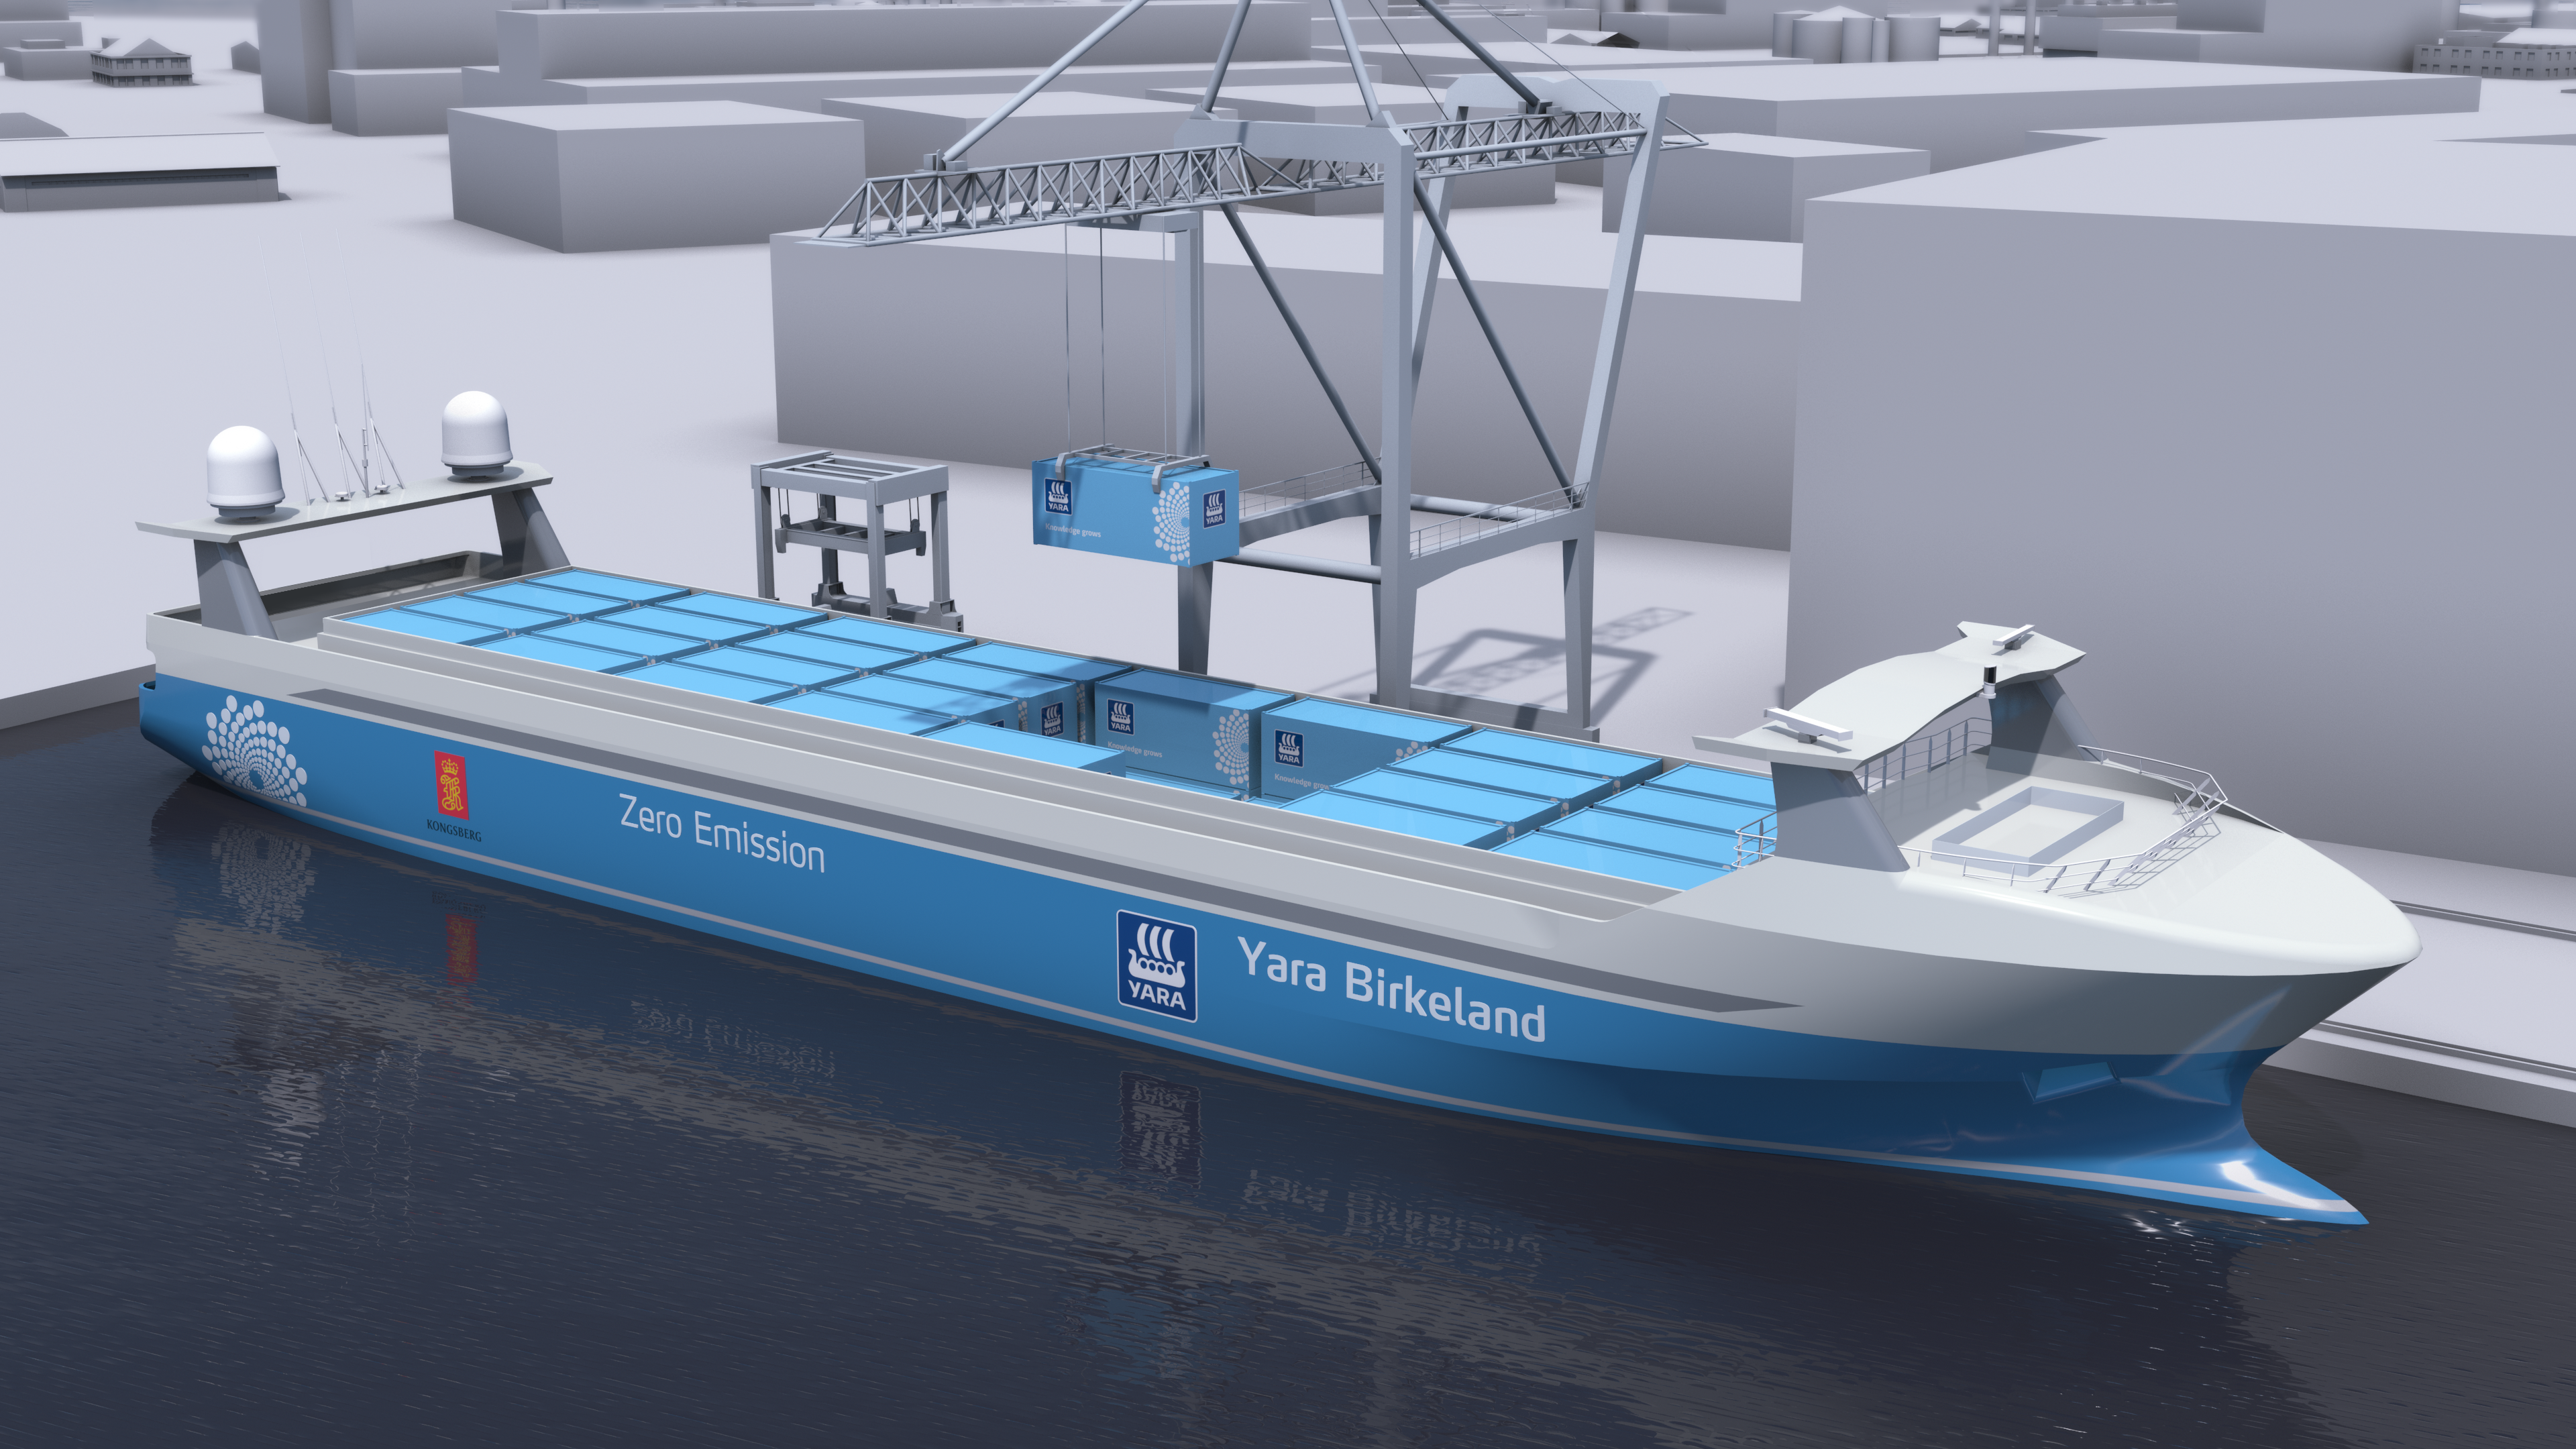
\includegraphics[width=\textwidth]{yara-birkeland.png}
	\caption{Render of Yara Birkeland}
	\label{fig:yara-birkeland}
\end{figure}

Other smaller projects are the development of Norwegian ferries, which are likely to start sailing automated from 2018, just like an automated shuttle service for offshore installations. A partly Dutch project is the Roboat, where a fleet of small pontoons will be used to solve problems on urban waterways. Such as transportation of people and goods, or creating temporary dynamic floating structures like bridges and stages. Roboat is a collaboration between AMS Institute and MIT.

Most of the previous projects focussed on developing a vessel, which has to operate in the current environment. The smart shipping challenge (SMASH) focusses on combining technological developments within different parts of the inland shipping industry in the Netherlands, such as bridges and terminals. This will help to steer ships remotely, enable the intelligent exchange of information, and the optimisation of waterway maintenance.
Good examples are the new vessels from Nedcargo and the Gouwenaar 3. These vessels will be able to transport more containers while reducing fuel consumption. This will not only be acquired by improving the hull shape and machinery, but also by sailing smarter. For example by optimising the speed, based on opening times for bridges and availability of the quay \cite{SMASH2017}. 

Also in the Netherlands are different partnerships working on the challenges of autonomous and unmanned shipping. The research conducted on communication and decision making will support one of these projects via Damen Shipyards and the Technical University of Delft. Where they partner with different European companies and research institutes, to develop a technology to deal with challenging environments and complex transport missions. Which is also applicable to other autonomous waterborne operations, such as inland waterways transport and coastal/inter-island short range ferry services.

Based on the projects mentioned above, are the most direct use cases: Local transport between factories and terminals and short sea shipping solutions. However, there might be more in the future, such as the usage of tugs as an additional actuator in dynamic positioning systems.

\section{Stakeholders}
When the ships mentioned in the previous section will sail, does not only dependent on the rate on which the technology can be developed. As stakeholders are there also regulatory bodies, such as \ac{IMO} and classification societies which need to incorporate autonomous vessels into their frameworks. 
The exploratory projects are important, as this will help them to prioritise the codes for different ship types. These codes include information on autonomy levels and how to certify unmanned vessels.

Another group of stakeholders are the shipbuilders, system integrators and suppliers for subsystems. These are responsible for technological development. More and more shipyards try to get involved, to gain knowledge on the development process. 
Also are there the companies from other industries, which see opportunities for products they already developed for planes or automotive. For example using computer vision, protocols for classifying systems and connecting ships.

The last, but probably most important are the customers, as technology will only be used if they can make money with it. More and more companies are convinced this is possible. These are not only the chartering companies but also their customers, such as Heineken, Yara and BHP.

\section{Challenges when combining unmanned and manned vessel}
\label{sec:challenges-future}
Based on the projects mentioned above it is clear that many projects work on different challenges. All challenges are related to the safe operation of unmanned vessels while optimising profit. For the technological challenge, is the most critical situations, when manned and unmanned vessels meet. Ship-to-ship communication is often necessary for those situations. Many of the projects so far, try to avoid these situations, as this will also result in fewer challenges for regulatory bodies. Also is technology for communication costly to develop, therefore is the aim to avoid communication where possible. The first step to accomplish this is to adjust the operational strategies for unmanned ships to avoid complex situations. This means that a strategy should be developed on how these ships can avoid communication. The easiest way is to operate only in area's where all risks are known. The best solution to enable a ship to operate everywhere is by avoiding the need for communication. This is achieved by taking decisions well in advance and making intentions clear. Still, some challenges are open, as ships cannot avoid all complex situations. For these cases, there must be a protocol which enables manned and unmanned ships to share the right information. Both of these issues have not been within the scope of the previously mentioned projects, or any other research \cite{Kooij2018}. 

\vspace{1.5cm}
\emph{In the next chapter} are factors discussed which influence the decision making process. We base these factors on challenges from previously mentioned projects and current research, where the decision model is a stepping stone.